\chapter{Affixation}
\label{Para_F}
The following sections present tables and figures which give the token frequencies by speakers, topics, and interlocutors for the affixes discussed in \sectref{Para_3.1}. The frequencies for prefix \textscItal{ter-} are given in Appendix \ref{Para_F.1}, for suffix \textit{-ang} in Appendix \ref{Para_F.2}, for prefix \textscItal{pe(n)-} in Appendix \ref{Para_F.3}, for prefix \textscItal{ber-} in Appendix \ref{Para_F.4}, for suffix \textit{-nya} in Appendix \ref{Para_F.5}, and for circumfix \textit{ke}\textit{-}/\textit{-}\textit{ang} in Appendix \ref{Para_F.6}.


\section[Prefix {\TER}-]{Prefix \textscItal{ter-}}
\label{Para_F.1}
The tables and figures give the token frequencies for \textscItal{ter-}prefixed words with bi- and \isi{monovalent} verbal bases.

\begin{table}
\begin{tabularx}{\textwidth}{Xrrrrrrrr}
\lsptoprule
& \multicolumn{4}{c}{Topics (\textsc{top})} & \multicolumn{3}{c}{ Interlocutors (\textsc{ilct})} &  Tokens\\\cmidrule(lr{\cmidrulekern}){2-5}\cmidrule(lr{\cmidrulekern}){6-8}
Speakers & \textsc{pol} & \textsc{edc} & \textsc{rel} & \textsc{low} & \textsc{+stat} & \textsc{\textminus stat} & \textsc{outsd} &  Total\\\midrule
\textsc{+edc-spk} &  6 &  10 &  10 &  15 &   --  &   --  &  9 &  50\\
\textsc{\textminus edc-spk} &  2 &  1 &  26 &   --  &  45 &  \textstyleChBold{23} &  6 &  103\\
\textstyleChBold{Total} &  8 &  11 &  36 &  15 &  45 &  \textstyleChBold{23} &  15 &  153\\
\lspbottomrule
\end{tabularx}
\caption[Tokens for \textsc{ter-}prefixed words with \isi{bivalent} verbal bases (38 items)]{Tokens for \textscItal{ter-}prefixed words with \isi{bivalent} verbal bases (38 items)}
\end{table}


\begin{figure}
\centering
%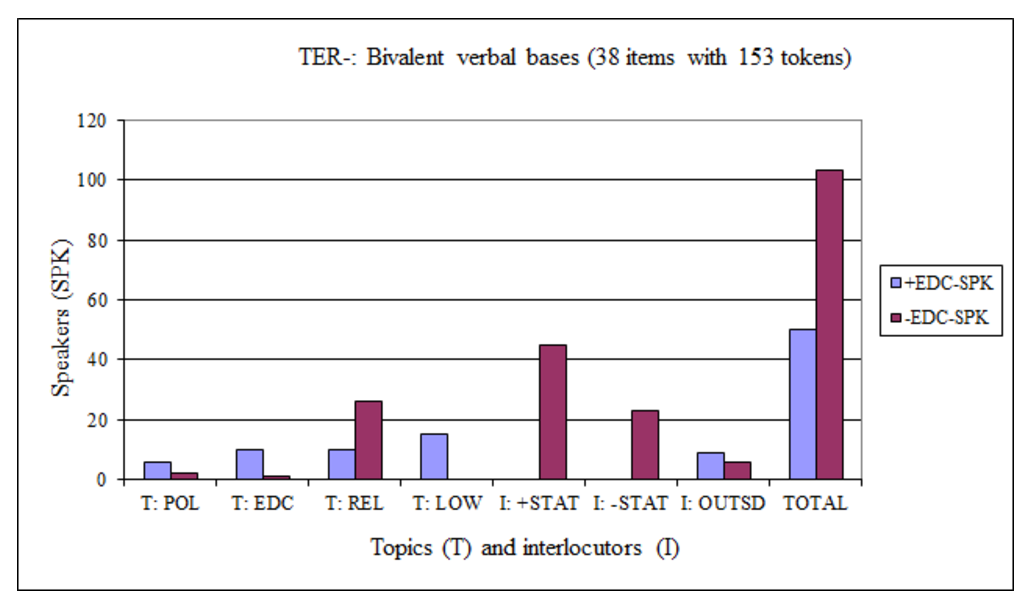
\includegraphics[scale=0.6]{./figures/Figure_A_F_1}
	\begin{tikzpicture}
	\begin{axis}[klugeaxis,title=\textscItal{ter}-: Bivalent verbal bases (38 items with 153 tokens)]
	\addplot[klugedots]	coordinates {(1,6)(2,10)(3,10)(4,15)(5,0)(6,0)(7,9)(8,50)};
	\addplot[klugelines] coordinates {(1,2)(2,1)(3,26)(4,0)(5,45)(6,23)(7,6)(8,103)};		
	\legend{\textsc{+edc-spk},\textsc{-edc-spk}}
	\end{axis}
	\end{tikzpicture}
\caption[Tokens for \textsc{ter-}prefixed words with \isi{bivalent} verbal bases]{Tokens for \textscItal{ter-}prefixed words with \isi{bivalent} verbal bases}\label{Figure_F.1}
\end{figure}


\begin{table}
\begin{tabularx}{\textwidth}{Xrrrrrrrr}
\lsptoprule
& \multicolumn{4}{c}{Topics (\textsc{top})} & \multicolumn{3}{c}{ Interlocutors (\textsc{ilct})} &  Tokens\\\cmidrule(lr{\cmidrulekern}){2-5}\cmidrule(lr{\cmidrulekern}){6-8}
Speakers & \textsc{pol} & \textsc{edc} & \textsc{rel} & \textsc{low} & \textsc{+stat} & \textsc{\textminus stat} & \textsc{outsd} &  Total\\\midrule
\textsc{+edc-spk} &  0 &  0 &  1 &  4 &   --  &   --  &  0 &  5\\
\textsc{\textminus edc-spk} &  0 &  1 &  5 &   --  &  2 &  \textstyleChBold{1} &  0 &  9\\
\textstyleChBold{Total} &  0 &  1 &  6 &  4 &  2 &  \textstyleChBold{1} &  0 &  14\\
\lspbottomrule
\end{tabularx}
\caption[Tokens for \textsc{ter-}prefixed words with \isi{monovalent} verbal bases (5 items)]{Tokens for \textscItal{ter-}prefixed words with \isi{monovalent} verbal bases (5 items)}
\end{table}




\begin{figure}
\centering
%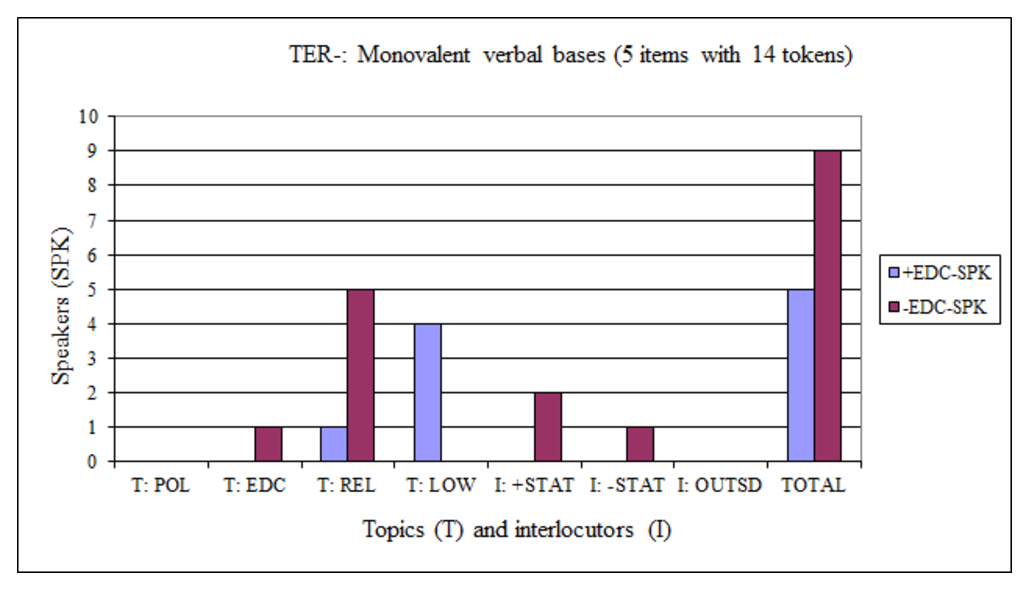
\includegraphics[scale=0.6]{./figures/Figure_A_F_2}
\begin{tikzpicture}
\begin{axis}[klugeaxis,title=\textscItal{ter}-: Monovalent verbal bases (5 items with 14 tokens)]
\addplot[klugedots]	coordinates {(1,0)(2,0)(3,1)(4,4)(5,0)(6,0)(7,0)(8,5)};
\addplot[klugelines] coordinates {(1,0)(2,1)(3,5)(4,0)(5,2)(6,1)(7,0)(8,9)};		
\legend{\textsc{+edc-spk},\textsc{-edc-spk}}
\end{axis}
\end{tikzpicture}
\caption[Tokens for \textsc{ter-}prefixed words with \isi{monovalent} verbal bases]{Tokens for \textscItal{ter-}prefixed words with \isi{monovalent} verbal bases}\label{Figure_F.2}
\end{figure}




\section[Suffix \textit{-ang}]{Suffix \textit{-ang}}
\label{Para_F.2}
The tables and figures give the token frequencies for \textit{-ang}{}-suffixed words with verbal, nominal, and \isi{numeral} bases.

\begin{table}
\begin{tabularx}{\textwidth}{Xrrrrrrrr}
\lsptoprule
& \multicolumn{4}{c}{Topics (\textsc{top})} & \multicolumn{3}{c}{ Interlocutors (\textsc{ilct})} &  Tokens\\\cmidrule(lr{\cmidrulekern}){2-5}\cmidrule(lr{\cmidrulekern}){6-8}
Speakers & \textsc{pol} & \textsc{edc} & \textsc{rel} & \textsc{low} & \textsc{+stat} & \textsc{\textminus stat} & \textsc{outsd} &  Total\\\midrule
\textsc{+edc-spk} &  30 &  26 &  15 &  46 &   --  &   --  &  75 &  192\\
\textsc{\textminus edc-spk} &  15 &  40 &  57 &   --  &  26 &  \textstyleChBold{80} &  3 &  211\\
\textstyleChBold{Total} &  45 &  66 &  62 &  46 &  26 &  \textstyleChBold{80} &  78 &  403\\
\lspbottomrule
\end{tabularx}
\caption[Tokens for \textit{-ang}{}-suffixed words with verbal bases (69 items)]{Tokens for \textit{-ang}{}-suffixed words with verbal bases (69 items)}
\end{table}

\begin{figure}
\centering
%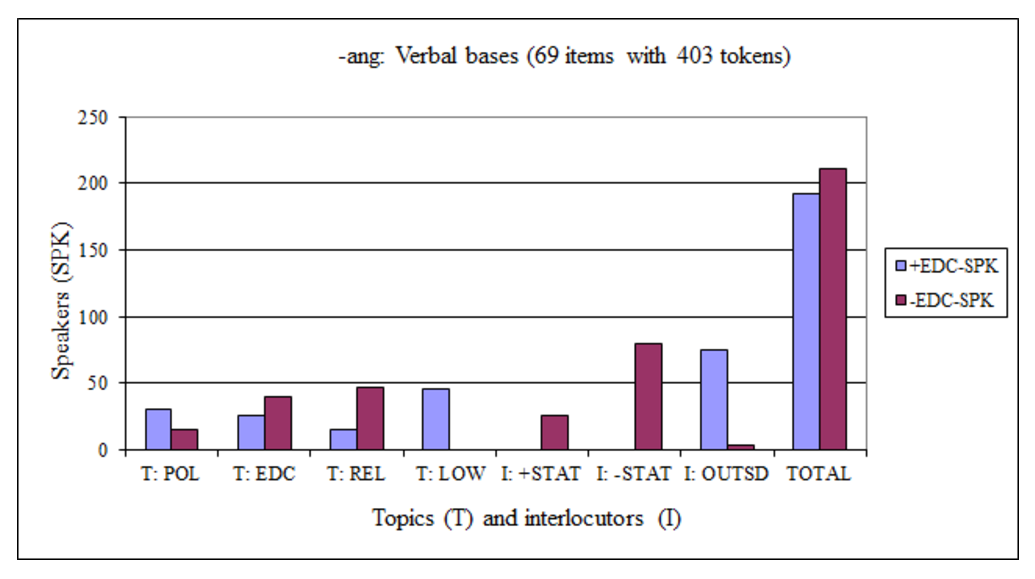
\includegraphics[scale=0.6]{./figures/Figure_A_F_3}
\begin{tikzpicture}
\begin{axis}[klugeaxis,y={},height={.5\textheight},title=\textit{-ang}: Verbal bases (69 items with 403 tokens)]
\addplot[klugedots]	coordinates {(1,30)(2,26)(3,15)(4,46)(5,0)(6,0)(7,75)(8,192)};
\addplot[klugelines] coordinates {(1,15)(2,40)(3,47)(4,0)(5,26)(6,80)(7,3)(8,211)};		
\legend{\textsc{+edc-spk},\textsc{-edc-spk}}
\end{axis}
\end{tikzpicture}
\caption[Tokens for \textit{-ang}{}-suffixed words with verbal bases]{Tokens for \textit{-ang}{}-suffixed words with verbal bases}\label{Figure_F.3}
\end{figure}




\begin{table}
\begin{tabularx}{\textwidth}{Xrrrrrrrr}
\lsptoprule
& \multicolumn{4}{c}{Topics (\textsc{top})} & \multicolumn{3}{c}{ Interlocutors (\textsc{ilct})} &  Tokens\\\cmidrule(lr{\cmidrulekern}){2-5}\cmidrule(lr{\cmidrulekern}){6-8}
Speakers & \textsc{pol} & \textsc{edc} & \textsc{rel} & \textsc{low} & \textsc{+stat} & \textsc{\textminus stat} & \textsc{outsd} &  Total\\\midrule
\textsc{+edc-spk} &  4 &  1 &  0 &  4 &   --  &   --  &  8 &  17\\
\textsc{\textminus edc-spk} &  3 &  0 &  6 &   --  &  1 &  \textstyleChBold{9} &  2 &  21\\
\textstyleChBold{Total} &  7 &  1 &  6 &  4 &  1 &  \textstyleChBold{9} &  10 &  38\\
\lspbottomrule
\end{tabularx}
\caption[Tokens for -\textit{ang}{}-suffixed words with nominal and \isi{numeral} bases (15 items)]{Tokens for -\textit{ang}{}-suffixed words with nominal and \isi{numeral} bases (15 items)}
\end{table}


\begin{figure}
\centering
%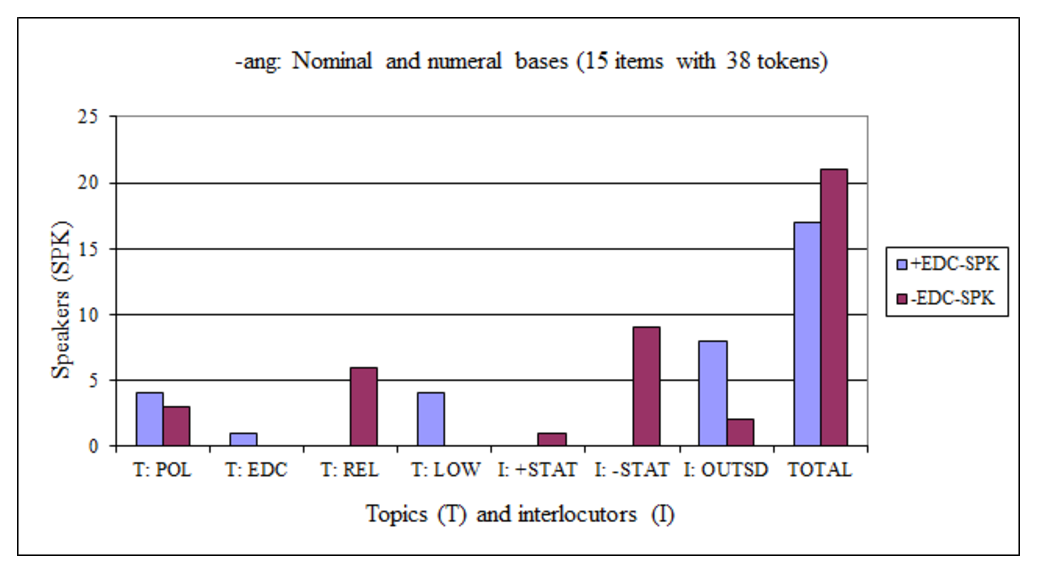
\includegraphics[scale=0.6]{./figures/Figure_A_F_4}
\begin{tikzpicture}
\begin{axis}[klugeaxis,title=\textit{-ang}: Nominal and \isi{numeral} bases (15 items with 38 tokens)]
\addplot[klugedots]	coordinates {(1,4)(2,1)(3,0)(4,4)(5,0)(6,0)(7,8)(8,17)};
\addplot[klugelines] coordinates {(1,3)(2,0)(3,6)(4,0)(5,1)(6,9)(7,2)(8,21)};		
\legend{\textsc{+edc-spk},\textsc{-edc-spk}}
\end{axis}
\end{tikzpicture}
\caption[Tokens for -\textit{ang}{}-suffixed items derived from nominal and \isi{numeral} bases]{Tokens for -\textit{ang}{}-suffixed items derived from nominal and \isi{numeral} bases}\label{Figure_F.4}
\end{figure}


\section[Prefix {\PEN}-]{Prefix \textscItal{pe(n)-}}
\label{Para_F.3}
The tables and figures give the token frequencies for \textscItal{pe(n)-}prefixed words with verbal and nominal bases.

\begin{table}
\begin{tabularx}{\textwidth}{Xrrrrrrrr}
\lsptoprule
& \multicolumn{4}{c}{Topics (\textsc{top})} & \multicolumn{3}{c}{ Interlocutors (\textsc{ilct})} &  Tokens\\\cmidrule(lr{\cmidrulekern}){2-5}\cmidrule(lr{\cmidrulekern}){6-8}
Speakers & \textsc{pol} & \textsc{edc} & \textsc{rel} & \textsc{low} & \textsc{+stat} & \textsc{\textminus stat} & \textsc{outsd} &  Total\\\midrule
\textsc{+edc-spk} &  37 &  6 &  3 &  19 &   --  &   --  &  11 &  76\\
\textsc{\textminus edc-spk} &  11 &  2 &  37 &   --  &  9 &  \textstyleChBold{18} &  0 &  77\\
\textstyleChBold{Total} &  48 &  8 &  40 &  19 &  9 &  \textstyleChBold{18} &  11 &  153\\
\lspbottomrule
\end{tabularx}
\caption[Tokens for \textsc{pe(n)-}prefixed words with verbal bases (29 items)]{Tokens for \textscItal{pe(n)-}prefixed words with verbal bases (29 items)}
\end{table}


\begin{figure}
\centering
%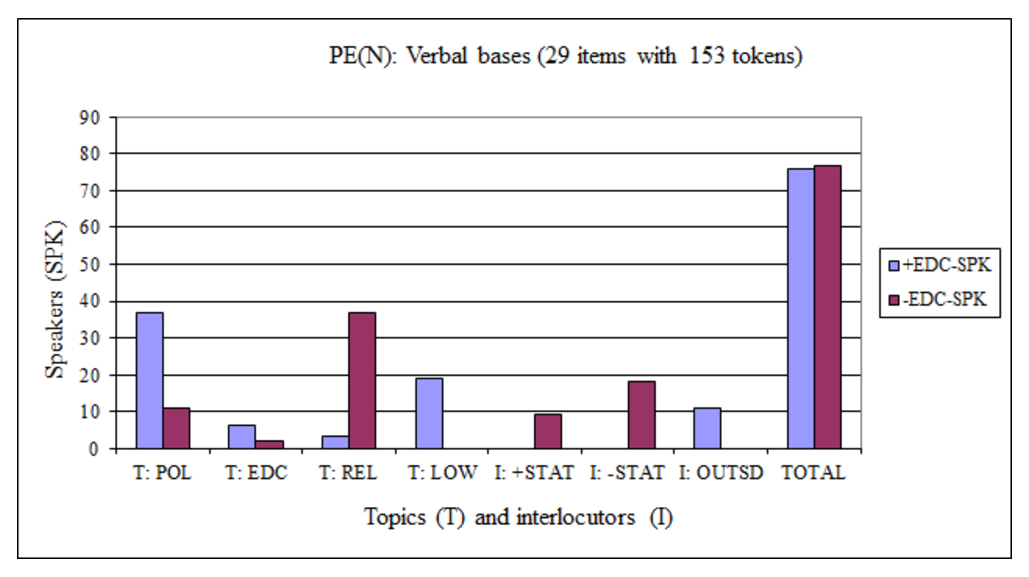
\includegraphics[scale=0.6]{./figures/Figure_A_F_5}
\begin{tikzpicture}
\begin{axis}[klugeaxis,title=\textscItal{pe(n)-}: Verbal bases (29 items with 153 tokens)]
\addplot[klugedots]	coordinates {(1,37)(2,6)(3,3)(4,19)(5,0)(6,0)(7,11)(8,76)};
\addplot[klugelines] coordinates {(1,11)(2,2)(3,37)(4,0)(5,9)(6,18)(7,0)(8,77)};		
\legend{\textsc{+edc-spk},\textsc{-edc-spk}}
\end{axis}
\end{tikzpicture}
\caption[Tokens for \textsc{pe(n)-}prefixed words with verbal bases]{Tokens for \textscItal{pe(n)-}prefixed words with verbal bases}\label{Figure_F.5}
\end{figure}

 
\begin{table}
\begin{tabularx}{\textwidth}{Xrrrrrrrr}
\lsptoprule
& \multicolumn{4}{l}{ Topics (\textsc{top})} & \multicolumn{3}{l}{ Interlocutors (\textsc{ilct})} &  Tokens\\
Speakers & \textsc{pol} & \textsc{edc} & \textsc{rel} & \textsc{low} & \textsc{+stat} & \textsc{\textminus stat} & \textsc{outsd} &  Total\\\midrule
\textsc{+edc-spk} &  10 &  0 &  12 &  5 &   --  &   --  &  0 &  27\\
\textsc{\textminus edc-spk} &  1 &  2 &  2 &   --  &  0 &  \textstyleChBold{1} &  0 &  6\\
\textstyleChBold{Total} &  11 &  2 &  14 &  5 &  0 &  \textstyleChBold{1} &  0 &  33\\
\lspbottomrule
\end{tabularx}
\caption[Tokens for \textsc{pe(n)-}prefixed words with nominal bases (5 items)]{Tokens for \textscItal{pe(n)-}prefixed words with nominal bases (5 items)}
\end{table}

\begin{figure}
\centering
%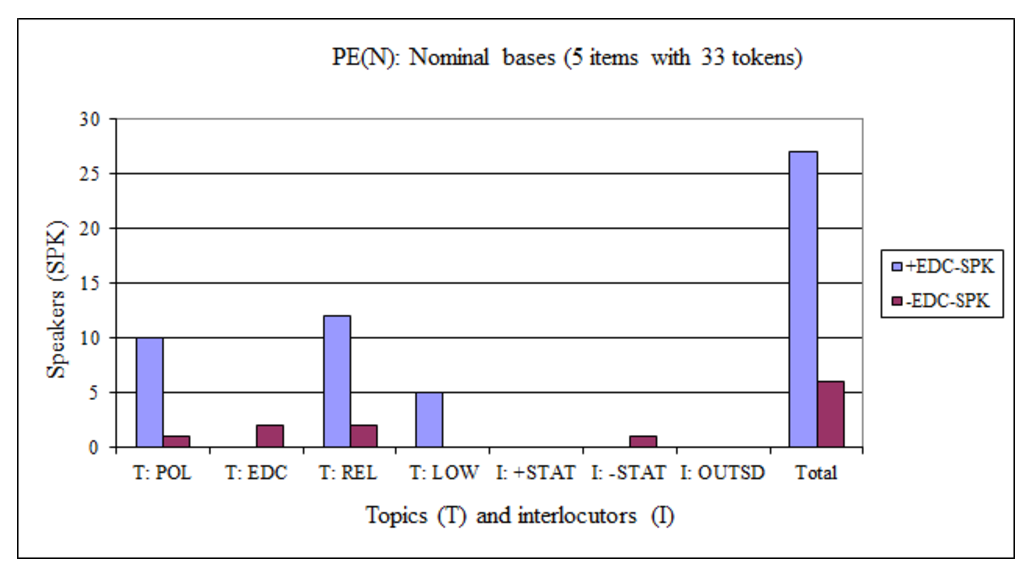
\includegraphics[scale=0.6]{./figures/Figure_A_F_6}
\begin{tikzpicture}
\begin{axis}[klugeaxis,title=\textscItal{pe(n)-}: Nominal bases (5 items with 33 tokens)]
\addplot[klugedots]	coordinates {(1,10)(2,0)(3,12)(4,5)(5,0)(6,0)(7,0)(8,27)};
\addplot[klugelines] coordinates {(1,1)(2,2)(3,2)(4,0)(5,0)(6,1)(7,0)(8,6)};		
\legend{\textsc{+edc-spk},\textsc{-edc-spk}}
\end{axis}
\end{tikzpicture}
\caption[Tokens for \textsc{pe(n)-}prefixed words with nominal bases]{Tokens for \textscItal{pe(n)-}prefixed words with nominal bases}\label{Figure_F.6}
\end{figure}
 
\clearpage
\section[Prefix {\BER}-]{Prefix \textscItal{ber-}}
\label{Para_F.4}
The tables and figures give the token frequencies for \textscItal{ber-}prefixed words with verbal, nominal, \isi{numeral}, and \isi{quantifier} bases.


\begin{table}
\begin{tabularx}{\textwidth}{Xrrrrrrrr}
\lsptoprule
& \multicolumn{4}{c}{Topics (\textsc{top})} & \multicolumn{3}{c}{ Interlocutors (\textsc{ilct})} &  Tokens\\\cmidrule(lr{\cmidrulekern}){2-5}\cmidrule(lr{\cmidrulekern}){6-8}
Speakers & \textsc{pol} & \textsc{edc} & \textsc{rel} & \textsc{low} & \textsc{+stat} & \textsc{\textminus stat} & \textsc{outsd} &  Total\\\midrule
\textsc{+edc-spk} &  7 &  22 &  9 &  12 &   --  &   --  &  7 &  57\\
\textsc{\textminus edc-spk} &  3 &  7 &  5 &   --  &  7 &  \textstyleChBold{8} &  7 &  37\\
\textstyleChBold{Total} &  10 &  29 &  14 &  12 &  7 &  \textstyleChBold{8} &  14 &  94\\
\lspbottomrule
\end{tabularx}
\caption[Tokens for \textsc{ber-}prefixed words with verbal bases (27 items]{Tokens for \textscItal{ber-}prefixed words with verbal bases (27 items)}
\end{table}

\begin{figure}
\centering
%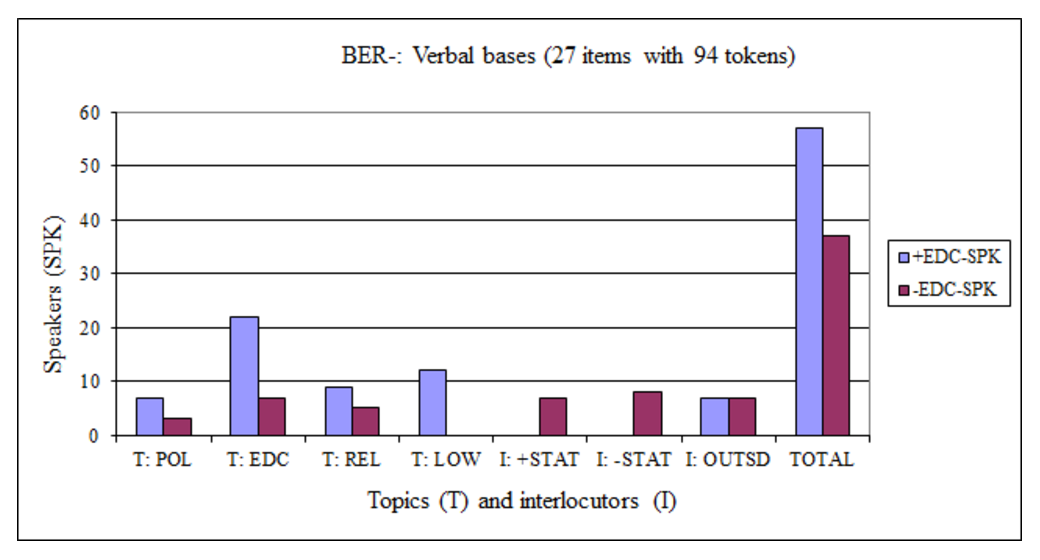
\includegraphics[scale=0.6]{./figures/Figure_A_F_7}
\begin{tikzpicture}
\begin{axis}[klugeaxis,title=\textscItal{ber}-: Verbal bases (27 items with 94 tokens)]
\addplot[klugedots]	coordinates {(1,7)(2,22)(3,9)(4,12)(5,0)(6,0)(7,7)(8,57)};
\addplot[klugelines] coordinates {(1,3)(2,7)(3,5)(4,0)(5,7)(6,8)(7,7)(8,37)};		
\legend{\textsc{+edc-spk},\textsc{-edc-spk}}
\end{axis}
\end{tikzpicture}
\caption[Tokens for \textsc{ber-}prefixed words with verbal bases]{Tokens for \textscItal{ber-}prefixed words with verbal bases}\label{Figure_F.7}
\end{figure}


\begin{table}
\begin{tabularx}{\textwidth}{Xrrrrrrrr}
\lsptoprule
& \multicolumn{4}{c}{Topics (\textsc{top})} & \multicolumn{3}{c}{ Interlocutors (\textsc{ilct})} &  Tokens\\\cmidrule(lr{\cmidrulekern}){2-5}\cmidrule(lr{\cmidrulekern}){6-8}
Speakers & \textsc{pol} & \textsc{edc} & \textsc{rel} & \textsc{low} & \textsc{+stat} & \textsc{\textminus stat} & \textsc{outsd} &  Total\\\midrule
\textsc{+edc-spk} &  13 &  9 &  11 &  6 &   --  &   --  &  7 &  46\\
\textsc{\textminus edc-spk} &  1 &  2 &  6 &   --  &  4 &  \textstyleChBold{8} &  3 &  24\\
\textstyleChBold{Total} &  14 &  11 &  17 &  6 &  4 &  \textstyleChBold{8} &  10 &  70\\
\lspbottomrule
\end{tabularx}
\caption[Tokens for \textsc{ber-}prefixed words with nominal, \isi{numeral}, and \isi{quantifier} bases (29 items)]{Tokens for \textscItal{ber-}prefixed words with nominal, \isi{numeral}, and \isi{quantifier} bases (29 items)}
\end{table}
\begin{figure}
\centering
%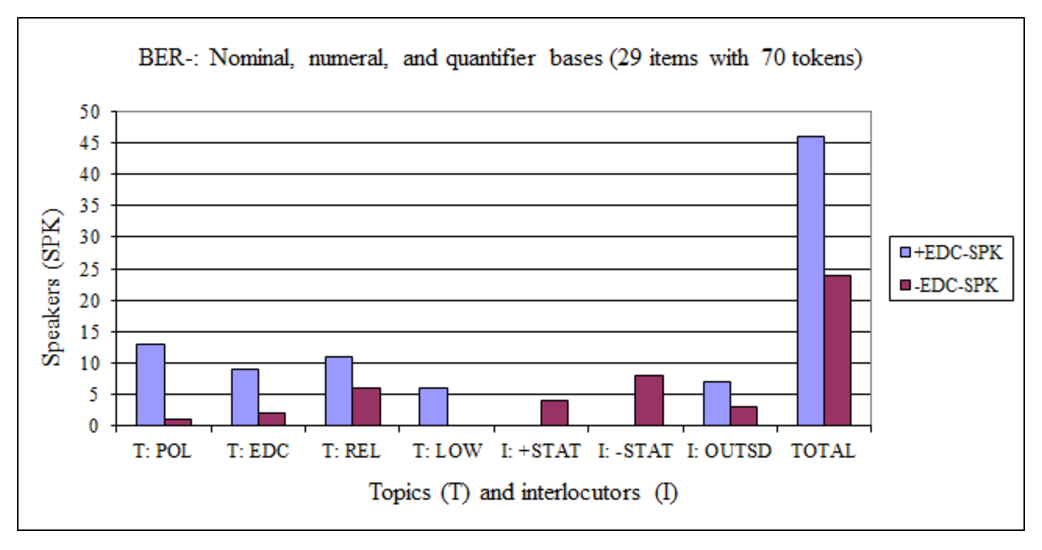
\includegraphics[scale=0.6]{./figures/Figure_A_F_8}
\resizebox{\textwidth}{!}{\begin{tikzpicture}
\begin{axis}[klugeaxis,title={\textscItal{ber}-: Nominal, \isi{numeral}, and \isi{quantifier} bases (29 items with 70 tokens)}]
\addplot[klugedots]	coordinates {(1,13)(2,9)(3,11)(4,6)(5,0)(6,0)(7,7)(8,46)};
\addplot[klugelines] coordinates {(1,1)(2,2)(3,6)(4,0)(5,4)(6,8)(7,3)(8,24)};		
\legend{\textsc{+edc-spk},\textsc{-edc-spk}}
\end{axis}
\end{tikzpicture}}
\caption[Tokens for \textsc{ber-}prefixed words with nominal, \isi{numeral}, and \isi{quantifier} bases]{Tokens for \textscItal{ber-}prefixed words with nominal, \isi{numeral}, and \isi{quantifier} bases}\label{Figure_F.8}
\end{figure}

\clearpage

\section[Suffix \textit{-nya}]{Suffix \textit{-nya}}
\label{Para_F.5}
The tables and figures give the token frequencies for \textit{-nya}{}-suffixed words with nominal, verbal, prepositional, and adverbial bases.


\begin{table}
\begin{tabularx}{\textwidth}{Xrrrrrrrr}
\lsptoprule
& \multicolumn{4}{c}{Topics (\textsc{top})} & \multicolumn{3}{c}{ Interlocutors (\textsc{ilct})} &  Tokens\\\cmidrule(lr{\cmidrulekern}){2-5}\cmidrule(lr{\cmidrulekern}){6-8}
Speakers & \textsc{pol} & \textsc{edc} & \textsc{rel} & \textsc{low} & \textsc{+stat} & \textsc{\textminus stat} & \textsc{outsd} &  Total\\\midrule
\textsc{+edc-spk} &  28 &  21 &  9 &  29 &   --  &   --  &  38 &  125\\
\textsc{\textminus edc-spk} &  12 &  5 &  14 &   --  &  20 &  \textstyleChBold{16} &  23 &  90\\
\textstyleChBold{Total} &  40 &  26 &  23 &  29 &  20 &  \textstyleChBold{16} &  61 &  215\\
\lspbottomrule
\end{tabularx}
\caption[Tokens for \textit{-nya}{}-suffixed words with nominal bases (81 items)]{Tokens for \textit{-nya}{}-suffixed words with nominal bases (81 items)}
\end{table}

\begin{figure}
\centering
%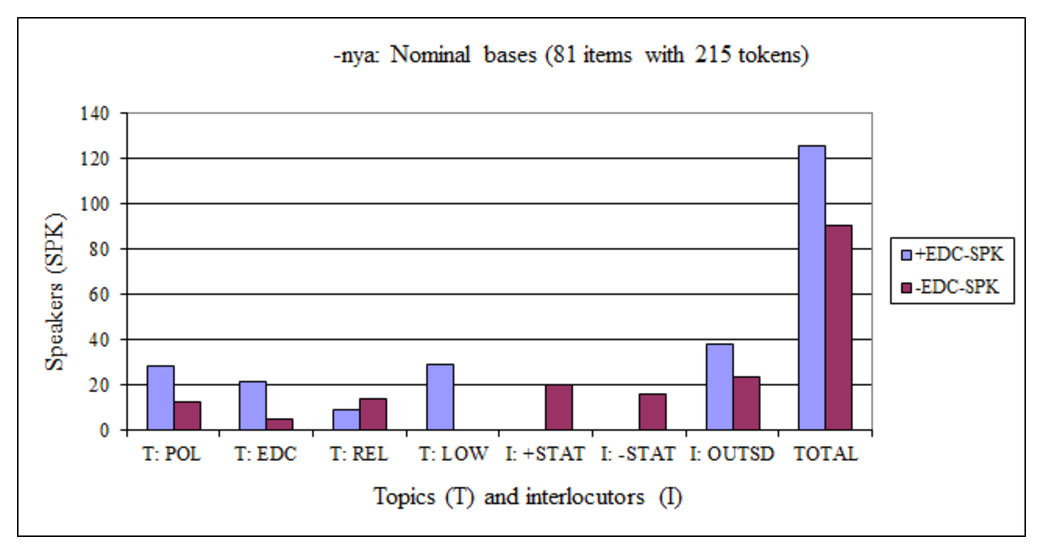
\includegraphics[scale=0.6]{./figures/Figure_A_F_9}
\begin{tikzpicture}
\begin{axis}[klugeaxis,title=\textit{-nya}: Nominal bases (81 items with 215 tokens)]
\addplot[klugedots]	coordinates {(1,28)(2,21)(3,9)(4,29)(5,0)(6,0)(7,38)(8,125)};
\addplot[klugelines] coordinates {(1,12)(2,5)(3,14)(4,0)(5,20)(6,16)(7,23)(8,90)};		
\legend{\textsc{+edc-spk},\textsc{-edc-spk}}
\end{axis}
\end{tikzpicture}
\caption[Tokens for \textit{-nya}{}-suffixed words with nominal bases]{Tokens for \textit{-nya}{}-suffixed words with nominal bases}\label{Figure_F.9}
\end{figure}


\begin{table} 
\begin{tabularx}{\textwidth}{Xrrrrrrrr}
\lsptoprule
& \multicolumn{4}{c}{Topics (\textsc{top})} & \multicolumn{3}{c}{ Interlocutors (\textsc{ilct})} &  Tokens\\\cmidrule(lr{\cmidrulekern}){2-5}\cmidrule(lr{\cmidrulekern}){6-8}
Speakers & \textsc{pol} & \textsc{edc} & \textsc{rel} & \textsc{low} & \textsc{+stat} & \textsc{\textminus stat} & \textsc{outsd} &  Total\\\midrule
\textsc{+edc-spk} &  5 &  14 &  3 &  11 &   --  &   --  &  16 &  49\\
\textsc{\textminus edc-spk} &  3 &  3 &  8 &   --  &  9 &  \textstyleChBold{8} &  2 &  33\\
\textstyleChBold{Total} &  8 &  17 &  11 &  11 &  9 &  \textstyleChBold{8} &  18 &  82\\
\lspbottomrule
\end{tabularx}
\caption[Tokens for \textit{-nya}{}-suffixed words with verbal bases (36 items)]{Tokens for \textit{-nya}{}-suffixed words with verbal bases (36 items)}
\end{table}

\begin{figure}
\centering
%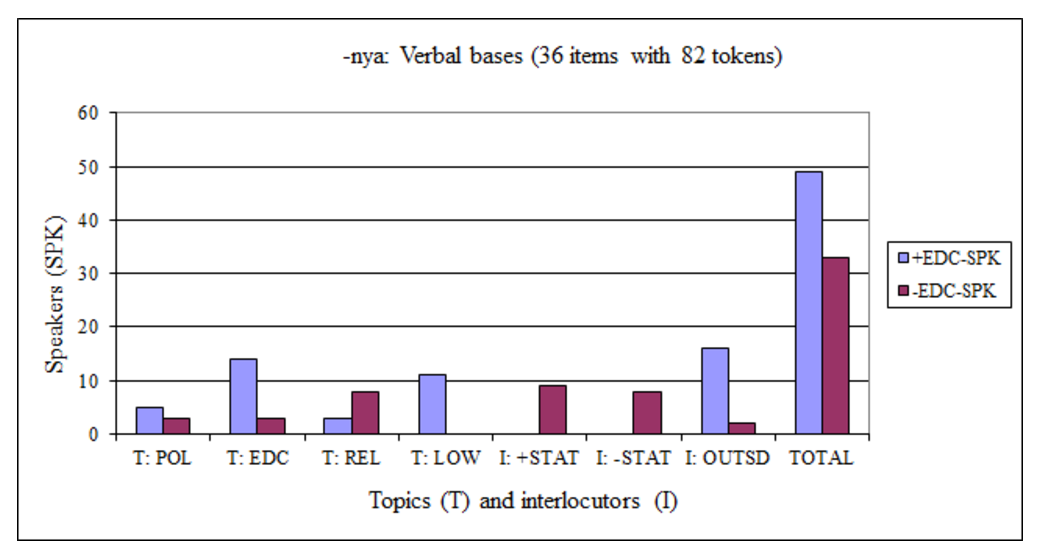
\includegraphics[scale=0.6]{./figures/Figure_A_F_10}
\begin{tikzpicture}
\begin{axis}[klugeaxis,title=\textit{-nya}: Verbal bases (36 items with 82 tokens)]
\addplot[klugedots]	coordinates {(1,5)(2,14)(3,3)(4,11)(5,0)(6,0)(7,16)(8,49)};
\addplot[klugelines] coordinates {(1,3)(2,3)(3,8)(4,0)(5,9)(6,8)(7,2)(8,33)};		
\legend{\textsc{+edc-spk},\textsc{-edc-spk}}
\end{axis}
\end{tikzpicture}
\caption[Tokens for \textit{-nya}{}-suffixed words with verbal bases]{Tokens for \textit{-nya}{}-suffixed words with verbal bases}\label{Figure_F.10}
\end{figure}


\begin{table}
\begin{tabularx}{\textwidth}{Xrrrrrrrr}
\lsptoprule
& \multicolumn{4}{c}{Topics (\textsc{top})} & \multicolumn{3}{c}{ Interlocutors (\textsc{ilct})} &  Tokens\\\cmidrule(lr{\cmidrulekern}){2-5}\cmidrule(lr{\cmidrulekern}){6-8}
Speakers & \textsc{pol} & \textsc{edc} & \textsc{rel} & \textsc{low} & \textsc{+stat} & \textsc{\textminus stat} & \textsc{outsd} &  Total\\\midrule
\textsc{+edc-spk} &  0 &  0 &  0 &  1 &   --  &   --  &  3 &  4\\
\textsc{\textminus edc-spk} &  1 &  3 &  6 &   --  &  1 &  \textstyleChBold{2} &  3 &  16\\
\textstyleChBold{Total} &  1 &  3 &  6 &  1 &  1 &  \textstyleChBold{2} &  6 &  20\\
\lspbottomrule
\end{tabularx}
\caption[Tokens for \textit{-nya}{}-suffixed words with prepositional and adverbial bases (5 items)]{Tokens for \textit{-nya}{}-suffixed words with prepositional and adverbial bases (5 items)}
\end{table}

\begin{figure}
\centering
%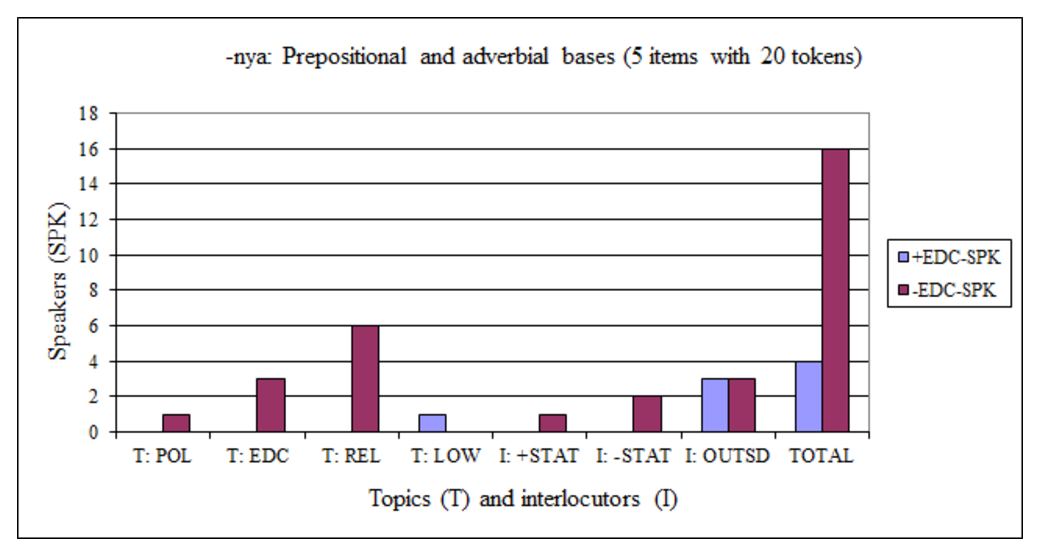
\includegraphics[scale=0.6]{./figures/Figure_A_F_11}
\begin{tikzpicture}
\begin{axis}[klugeaxis,title=\textit{-nya}: Prepositional and adverbial bases (5 items with 20 tokens)]
\addplot[klugedots]	coordinates {(1,0)(2,0)(3,0)(4,1)(5,0)(6,0)(7,3)(8,4)};
\addplot[klugelines] coordinates {(1,1)(2,3)(3,6)(4,0)(5,1)(6,2)(7,3)(8,16)};		
\legend{\textsc{+edc-spk},\textsc{-edc-spk}}
\end{axis}
\end{tikzpicture}
\caption[Tokens for \textit{-nya}{}-suffixed words with prepositional and adverbial base]{Tokens for \textit{-nya}{}-suffixed words with prepositional and adverbial bases}\label{Figure_F.11}
\end{figure}


\section[Circumfix \textit{ke-}/\textit{-ang}]{Circumfix \textit{ke-}/\textit{-ang}}
\label{Para_F.6}
The tables and figures give the token frequencies for \textit{ke-}/\textit{-ang}{}-circumfixed words with verbal, nominal, \isi{numeral}, and \isi{quantifier} bases.

\begin{table}
\begin{tabularx}{\textwidth}{Xrrrrrrrr}
\lsptoprule
& \multicolumn{4}{c}{Topics (\textsc{top})} & \multicolumn{3}{c}{ Interlocutors (\textsc{ilct})} &  Tokens\\\cmidrule(lr{\cmidrulekern}){2-5}\cmidrule(lr{\cmidrulekern}){6-8}
Speakers & \textsc{pol} & \textsc{edc} & \textsc{rel} & \textsc{low} & \textsc{+stat} & \textsc{\textminus stat} & \textsc{outsd} &  Total\\\midrule
\textsc{+edc-spk} &  14 &  36 &  13 &  38 &   --  &   --  &  43 &  144\\
\textsc{\textminus edc-spk} &  5 &  19 &  16 &   --  &  35 &  \textstyleChBold{12} &  8 &  95\\
\textstyleChBold{Total} &  19 &  55 &  29 &  38 &  35 &  \textstyleChBold{12} &  51 &  239\\
\lspbottomrule
\end{tabularx}
\caption[Tokens for \textit{ke-}/\textsc{-ang}{}-circumfixed words with verbal bases (57 items)]{Tokens for \textit{ke-}/\textit{-ang}{}-circumfixed words with verbal bases (57 items)}
\end{table}

\begin{figure}
\centering
%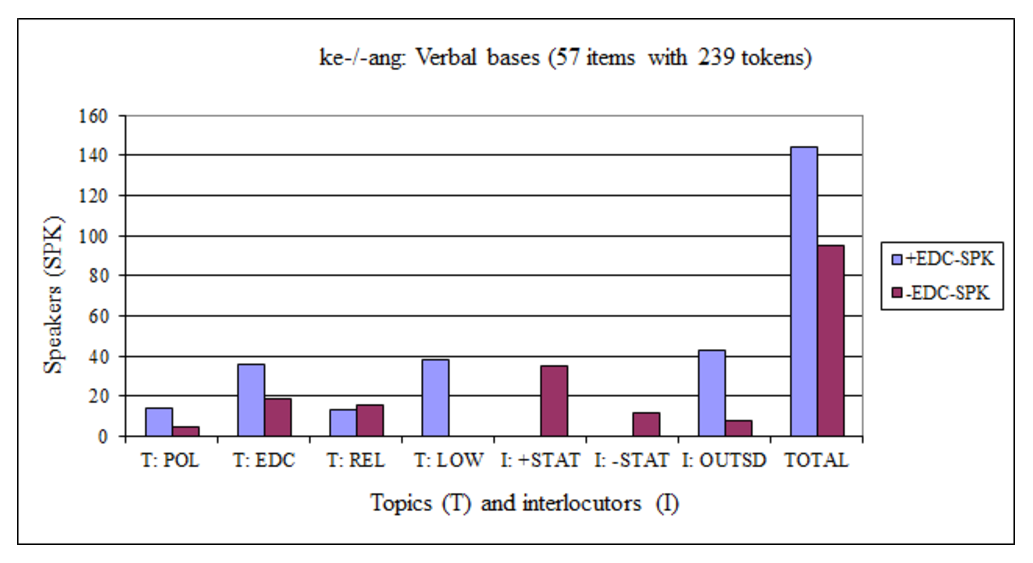
\includegraphics[scale=0.6]{./figures/Figure_A_F_12}
\begin{tikzpicture}
\begin{axis}[klugeaxis,title=\textit{ke}\textscItal{-}/\textscItal{-}\textit{ang}: Verbal bases (57 items with 239 tokens)]
\addplot[klugedots]	coordinates {(1,14)(2,36)(3,13)(4,38)(5,0)(6,0)(7,43)(8,144)};
\addplot[klugelines] coordinates {(1,5)(2,19)(3,16)(4,0)(5,35)(6,12)(7,8)(8,95)};		
\legend{\textsc{+edc-spk},\textsc{-edc-spk}}
\end{axis}
\end{tikzpicture}
\caption[Tokens for \textit{ke-}/\textsc{-ang}{}-circumfixed words with verbal bases]{Tokens for \textit{ke-}/\textit{-ang}{}-circumfixed words with verbal bases}\label{Figure_F.12}
\end{figure}


\begin{table}
\begin{tabularx}{\textwidth}{Xrrrrrrrr}
\lsptoprule
& \multicolumn{4}{c}{Topics (\textsc{top})} & \multicolumn{3}{c}{ Interlocutors (\textsc{ilct})} &  Tokens\\\cmidrule(lr{\cmidrulekern}){2-5}\cmidrule(lr{\cmidrulekern}){6-8}
Speakers & \textsc{pol} & \textsc{edc} & \textsc{rel} & \textsc{low} & \textsc{+stat} & \textsc{\textminus stat} & \textsc{outsd} &  Total\\\midrule
\textsc{+edc-spk} &  2 &  10 &  1 &  0 &   --  &   --  &  2 &  15\\
\textsc{\textminus edc-spk} &  2 &  1 &  0 &   --  &  0 &  \textstyleChBold{1} &  0 &  4\\
\textstyleChBold{Total} &  4 &  11 &  1 &  0 &  0 &  \textstyleChBold{1} &  2 &  19\\
\lspbottomrule
\end{tabularx}
\caption[Tokens for \textit{ke-}/\textsc{-ang}{}-circumfixed words with nominal, \isi{numeral}, and \isi{quantifier} bases (8 items)]{Tokens for \textit{ke-}/\textit{-ang}{}-circumfixed words with nominal, \isi{numeral}, and \isi{quantifier} bases (8 items)}
\end{table}

\begin{figure}
\centering
%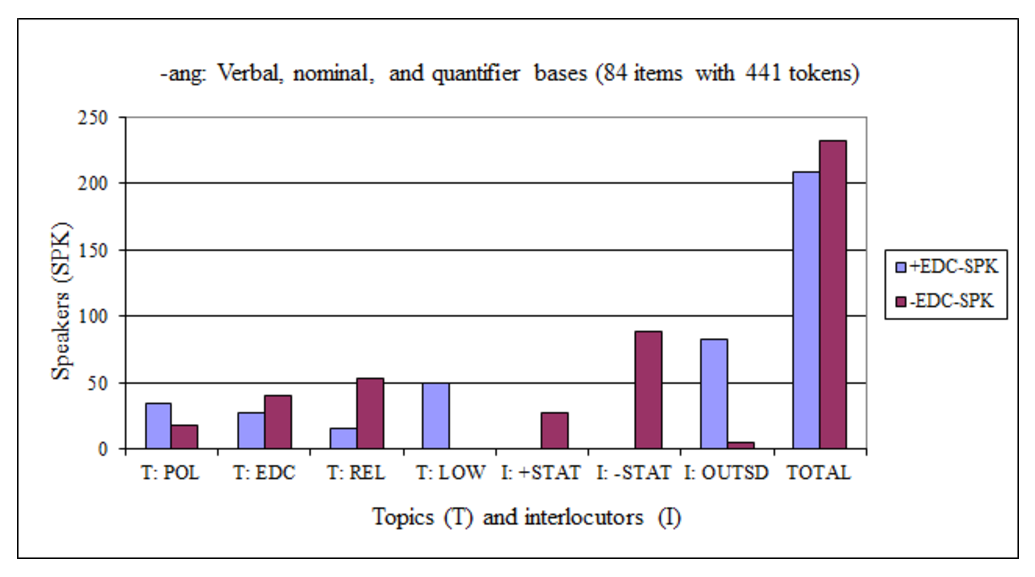
\includegraphics[scale=0.6]{./figures/Figure_A_F_13}
\begin{tikzpicture}
\begin{axis}[klugeaxis,title=\textit{ke}\textscItal{-}/\textscItal{-}\textit{ang}: {Verbal, nominal, and \isi{quantifier} bases (84 items with 441 tokens)}]
\addplot[klugedots]	coordinates {(1,2)(2,10)(3,1)(4,0)(5,0)(6,0)(7,2)(8,15)};
\addplot[klugelines] coordinates {(1,2)(2,1)(3,0)(4,0)(5,0)(6,1)(7,0)(8,4)};		
\legend{\textsc{+edc-spk},\textsc{-edc-spk}}
\end{axis}
\end{tikzpicture}
\caption[Tokens for \textit{ke-}/\textsc{-ang}{}-circumfixed words with nominal, \isi{numeral}, and \isi{quantifier} bases]{Tokens for \textit{ke-}/\textit{-ang}{}-circumfixed words with nominal, \isi{numeral}, and \isi{quantifier} bases}\label{Figure_F.13}
\end{figure}

